%%
\documentclass[%
]{article}


\usepackage[14pt]{extsizes} % для того чтобы задать нестандартный 14-ый размер шрифта
\usepackage[left=20mm, top=15mm, right=15mm, bottom=30mm, footskip=15mm]{geometry}
\geometry{a4paper}

% \usepackage{apacite}

\usepackage[utf8]{inputenc}

\usepackage{polyglossia}
\setdefaultlanguage{english}
\setotherlanguages{english}

\usepackage[style=apa, citestyle=numeric]{biblatex}
\usepackage{graphicx}

\DeclareFieldFormat{labelnumberwidth}{\mkbibbrackets{#1}}

\defbibenvironment{bibliography}
  {\list
     {\printtext[labelnumberwidth]{%
      \printfield{labelprefix}%
      \printfield{labelnumber}}}
     {\setlength{\labelwidth}{\labelnumberwidth}%
      \setlength{\leftmargin}{\labelwidth}%
      \setlength{\labelsep}{\biblabelsep}%
      \addtolength{\leftmargin}{\labelsep}%
      \setlength{\itemsep}{\bibitemsep}%
      \setlength{\parsep}{\bibparsep}}%
      \renewcommand*{\makelabel}[1]{\hss##1}}
  {\endlist}
  {\item}

%\captionsetup[listing]{name=Листинг}

\setmainfont[Ligatures=TeX,Scale=MatchLowercase]{CMU Serif}
\setsansfont[Ligatures=TeX,Scale=MatchLowercase]{CMU Sans Serif}
\setmonofont[Scale=MatchLowercase]{CMU Typewriter Text}

% CMU Serif
\newfontfamily\cyrillicfont%
[Script=Cyrillic,Ligatures=TeX,Scale=MatchLowercase]%
{CMU Serif}

% CMU Sans Serif
\newfontfamily\cyrillicfontsf%
[Script=Cyrillic,Ligatures=TeX,Scale=MatchLowercase]%
{CMU Sans Serif}

% CMU Typewriter Text
\newfontfamily\cyrillicfonttt%
[Script=Cyrillic,Scale=MatchLowercase]%
{CMU Typewriter Text}

%%% One can fix some overfulls
\sloppy

%% Minted listings support
%% Need pygment <http://pygments.org/> <http://pypi.python.org/pypi/Pygments>
%\usepackage[newfloat]{minted}
\usepackage{minted}
%% auto break lines
\setminted{breaklines=true}

%\usepackage{caption}

%\newenvironment{code}{\captionsetup{type=listing}}{}
%\SetupFloatingEnvironment{listing}{name=Листинг}

\addbibresource{main.bib}

%% end of the preamble, start of the body of the document source.
\begin{document}

\selectlanguage{english}

\title{none}

% НАЧАЛО ТИТУЛЬНОГО ЛИСТА
\begin{titlepage}

  \begin{center}
  \hfill \break
  \large{Peoples’ Friendship University of Russia}\\
  \large{named after Patrice Lumumba}\\
  \normalsize{Faculty of Physics and Mathematics and Natural Sciences}\\ 
  \normalsize{Department of Mathematical Modeling and Artificial Intelligence}\\

  \vspace*{\fill}

  % \begin{flushright}
  %   \large{Утверждаю}\\
  %   \normalsize{Заведующий кафедрой} 
  %   \normalsize{математического \\ моделирования и \\ искусственного интеллекта \\} 
  %   \underline{\phantom{signature signature}} Малых М.Д. \\
  %   <<\underline{\phantom{day}}>> \underline{\phantom{month month}} 2025 г.
  %   \end{flushright}
 
  \vspace*{\fill}
  \textbf{\textit{
    Simulation of Robot Swarm Behavior in a Wireless Mesh Network
  }}

  \vspace*{\fill}

  \end{center}
   
   \begin{flushright}
    Word Count: 4816 \\
    Student: \\
    Group NPIbd-01-21\\
    Student ID \textnumero{}: 1032212280 \\
    Generalov Daniil \\
    \underline{\phantom{signature signature}} \\
    << \underline{\phantom{day}} >> \underline{\phantom{month month}} 2025
   \end{flushright}

   \vspace*{\fill}

   \begin{flushright}
    Argument Consultant: \\
    Associate Professor \\
    Vinogradov A. N. \\
    \underline{\phantom{signature signature}} \\
    << \underline{\phantom{day}} >> \underline{\phantom{month month}} 2025
   \end{flushright}

   \vspace*{\fill}

   \begin{flushright}
    Style and Language Consultant: \\
    Senior Lecturer \\
    Kozhukhova Yu.V. \\
    \underline{\phantom{signature signature}} \\
    << \underline{\phantom{day}} >> \underline{\phantom{month month}} 2025
   \end{flushright}


   \begin{center} \textbf{Moscow} \\ 2025 \end{center}
  \thispagestyle{empty} % выключаем отображение номера для этой страницы
   
  \end{titlepage}
   % КОНЕЦ ТИТУЛЬНОГО ЛИСТА
  
  \newpage



% %%
% %% Rights management information.
% %% CC-BY is default license.
% \copyrightyear{2025}
% \copyrightclause{Copyright for this paper by its authors.
%   Use permitted under Creative Commons License Attribution 4.0
%   International (CC BY 4.0).}

% %%
% %% This command is for the conference information
% % \conference{Information and Telecommunication Technologies and Mathematical Modeling of High-Tech Systems 2025 (ITTMM 2025), Moscow, April 07--11, 2025}

% %%
% %% The "title" command
% \title{Wireless mesh network simulator for mobile robots}
% \title[mode=trans]{Wireless mesh network simulator for mobile robots}

% % \tnotemark[1]
% % \tnotetext[1]{You can use this document as the template for preparing your publication. We recommend using the latest version of the ittmm style.}

% %%
% %% The "author" command and its associated commands are used to define
% %% the authors and their affiliations.
% \author[1]{Daniil M. Generalov}[%
% trans={Даниил М. Генералов},
% orcid=0000-0002-2337-1176,
% email=1032212280@pfur.ru,
% %url=https://yamadharma.github.io/,
% ]
% % \cormark[1]

% \address[1]{Российский университет дружбы народов, ул. Миклухо-Маклая, д. 6, Москва, 117198, Российская Федерация}

% \author[1]{Andrei N. Vinogradov}[%
% trans={Андрей Н. Виноградов},
% email=vinogradov-an@rudn.ru,
% orcid=0000-0002-3349-8859,
% ]

%%% Footnotes
% \cortext[1]{Автор, отвечающий за публикацию.}

%%
%% The abstract is a short summary of the work to be presented in the
%% article.
\begin{abstract}
  This work presents a wireless mesh network simulator
  for development and testing of routing algorithms
  in wireless mesh-networks on mobile robots.
  Using this simulator,
  one can study the behavior of these robots
  under different radio conditions,
  which are difficult to simulate on physical equipment.
  The code written for the simulator can be used on physical microcontrollers
  without changes.
  The ability for robots to move in a rectangular grid
  and simultaneously make or break connections
  is an approach that is difficult to replicate in existing network simulation tools.
\end{abstract}

\newpage

\tableofcontents

\newpage


%%
%% Keywords. The author(s) should pick words that accurately describe
%% the work being presented. Separate the keywords with commas.
% \begin{keywords}
%   mesh-network \sep
%   MANET \sep
%   маршрутизация \sep
%   симулятор
% \end{keywords}

%% This command processes the author and affiliation and title
%% information and builds the first part of the formatted document.
% \maketitle

\section{Introduction}
\label{sec:intro}


The topic of this work is wireless mesh networks and their use in mobile robotics,
specifically for the use in the development and testing of routing algorithms,
then using them for multi-agent planning.

We have developed a new simulator for wireless mesh networks
that allows for the study of the behavior of mobile robots
in such networks under different radio conditions.
The \textbf{relevance} of this work
is increased because
both mobile robotics and mesh networks
are areas of interest in research and in industry.

There have been several simulators developed
specifically for wireless mesh networks,
but those aren't linked to any particular hardware implementation.
The \textbf{novelty} of our simulator is that
it allows the same code to be used
as a simulator script
as well as on physical microcontrollers,
increasing portability.
(TODO: add small literature review, referencing existing work)

We \textbf{aim} to develop the simulator
for wireless mesh networks on mobile robots
that is able to simulate
various network conditions
and how they affect
different aspects of the routing protocol's performance.

To do this we had to solve several \textbf{tasks}.
First, the simulator framework needed to be defined
(such as the APIs for user code. and matters of geometry and radio propagation rules).
Then, we had to actually implement the simulator and
have robots that can move and send messages to each other.
Finally, we need to write code related to the robot movement
and implement the actual protocols.

The simulator application can then be used
to help us resolve our \textbf{hypothesis},
which is that application-specific routing algorithms
perform better in mesh network conditions
than standard routing algorithms.

The \textbf{methods and tools} employed while developing this application
are standard in the field of software development.
Of particular interest is the use of
the Rust programming language,
which enables writing safe and efficient code
that can be compiled across platforms
(which enables the novelty of our work here).


\subsection{Wireless mesh networks}
Wireless mesh networks (such as MANETs, \emph{Mobile Ad-hoc Networks}) differ from traditional radio networks
in that they do not have a central router (such as a Wi-Fi AP or cellular base station -- this is commonly referred to as a \emph{hub-and-spoke design});
instead, each client in the network also acts as a router for its neighbors.

This principle is similar to how walkie-talkies operate:
each walkie-talkie can transmit a signal to those receivers that are within its range.
In such a network, information can travel further than the range of a single signal through relaying:
if Alice wants to send a message to Charlie, but Alice is too far away from him,
she can send her message to Bob, and Bob can relay the message further --
either directly to Charlie if he is within his range, or to someone else who is closer to Charlie.

This method of connectivity resembles the broad structure of the internet:
there are also no central routers, and instead, each Autonomous System (AS) has \emph{peering} connections with other ASes.
For this, the administrators of two networks connect their routers to each other and configure their networks
so that both sides can deliver their packets through the other AS.

Thus, the networks of various organizations form a global network.
Autonomous Systems exchange information about which other ASes
are available to them using BGP (Border Gateway Protocol),
and based on this information, their routers decide where to send the incoming traffic.

The structure in a wireless mesh network is somewhat analogous to the AS structure on the internet.
However, there is one important difference: the configuration of peer connections between ASes is done manually
with the mutual consent of the administrators of each AS, and requires the establishment of a physical connection
and configuring the routers within the AS.
In contrast, in a wireless mesh network, devices can move relative to each other
and change their network configuration dynamically, so the establishment of physical connections
between devices and the exchange of information must occur without human intervention.

An additional complexity arises from the fact that wireless mesh networks are often most economical to deploy in situations
where each device has limited computational resources. Autonomous Systems,
especially large ones, consist of powerful routers that have the capability to store the entire map of the global
internet in RAM and quickly use it for route finding.
By contrast, wireless mesh networks are used in situations
where there is a need to utilize simpler hardware, such as smartphones or even microcontrollers:
they do not always have the ability to store a complete map of their network, and therefore must employ approaches to work with limited resources.
In many such deployments, it is not even practical to add a central node that would know the entire map of the network:
for instance, if it's an IoT application, then this would require that the consumer buys an additional hardware device
that serves no discernable purpose~\footnote{In many IoT ecosystems, there is in fact a powerful device available:
it is typically called a hub, such as a "Zigbee hub", and it has connections to the internet.
Typically this device is combined with some extra functionality, such as a smart speaker,
which lets the consumer know that it requires internet connectivity
and thus lets the smaller IoT devices talk to the wider world through the hub.}.

Mesh networks are more challenging to develop because they require
addressing coordination problems 
(like avoiding network loops, or ensuring data consistency as in the Byzantine Generals Problem)
on a network-wide scale, while each node only has a local view of the network --
having a centralized management infrastructure, like traditional network hardware does, greatly simplifies this process.
However, mesh networks are very useful in situations where fixed networks are unavailable or unreliable:
for example, during search and rescue operations or when there is a disruption in power infrastructure.

There are already projects for simulating routing in fixed networks:
for example, GNS3, OMNeT++~\cite{9181563}, and Cisco PacketTracer.
However, using such projects to simulate a wireless mesh network,
especially one based on mobile robots, is challenging:
these programs expect the user to configure all wired connections during modeling,
and dynamically changing connections in them is more complex or impossible, and in any case requires manual input.

There are also some algorithms for routing that are specialized for mesh networks
(for example, OLSR and B.A.T.M.A.N~\cite{DBLP:journals/corr/abs-1901-02298}).
With a simulator like ours, it is possible to test the resilience of these algorithms
to changing conditions, identify potential pathological cases,
and explore possible improvements in a controlled environment.

\subsection{Multi-Agent Planning}

Multi-Agent Planning (MAP) is an extension of the classical planning problem to multiple agents.

The standard planning problem consists of two parts:
the \emph{domain} and the \emph{problem}. In the domain, the types of objects that exist,
the predicates that can be used in the problem, and the possible actions (each defined as a combination of preconditions and postconditions) are described.
For example, a domain can specify that there exist locations, robots and boxes, that robots and boxes can be positioned at locations,
and that robots can move and pick up the boxes.

In the problem, a specific set of objects is described,
along with the initial state of the world (as a set of predicates),
and the goal state -- a set of predicates such that after executing the plan,
the world will satisfy these predicates.
For example, a problem can specify that there is a robot that's currently
in the warehouse, that there is a truck that is reachable from the warehouse,
that there are three boxes in the warehouse,
and that the goal is that the three boxes need to end up in the truck while the robot is in the warehouse.

There are several different definitions of the MAP problem.
The most common definition (according to~\cite{doi:10.3233/MGS-2009-0133}), which we use in this project,
is that all agents share a common domain and common information about the initial state,
but they may have different goals.
Agents cannot communicate their goals to each other (for example because they may be secret);
instead, they propose plans, and other agents can either accept or reject them.

An additional complication arises when the information about the initial state is incomplete,
and observations may contradict the data in the state.
In such cases, agents must pause the execution of the plan and discuss what to do next:
this new information may necessitate a re-evaluation of the plan.

In the context of this work, the mesh network is created to facilitate communication between robots
that are solving a multi-agent planning problem.
In general, the module for working with the mesh network can be used independently,
but in this work we are also interested in the interaction between these components:
for example, a robot may refuse to execute a plan that would result in it becoming isolated from other robots.

\section{Development} 
\label{sec:base-section}

\subsection{Wireless Hardware}

One of the first decisions that needed to be made during the development of this project was:
which physical wireless hardware do we use as a model for developing the simulator~\footnote{The development results, including the source code for the simulator and this article, can be found online at \texttt{https://github.com/rudn-lab/planning-mesh-swarm}.}.
In this, we considered several factors:

\begin{enumerate}
  \item Framing: The task of working with physical (L1 and L2 according to the OSI model) frames has
  already been extensively solved by existing data transmission protocols,
  so we want to use a module that provides access to ready-made
  frames or packets and handles deriving them from the radio signal.
  
  \item Link-layer detection: Since some routing protocols
  (e.g., OSPF and its enhancements~\cite{rfc5614}) require the network nodes to understand when their
  connection with a neighbor is working or not, we want hardware that already has this capability in some form.
  (If this is not available at the hardware level, it can be implemented virtually by sending ping messages to each other, but this adds complexity to our code.)
  
  \item Identification: To avoid the need to create and verify
  unique identities for the nodes in our business logic,
  we want the modules to have their own unique identifier (e.g., a MAC address)
  and to automatically transmit it with each message: this way, we do not have to write code to distinguish one sender from another.
  
  \item Cost: We have limited financial resources for this project,
  so the modules we choose for physical implementation must constitute
  a small portion of the overall budget. In particular, this makes modules like
  LoRa unsuitable, even though they would be a good choice for practical implementations.
\end{enumerate}

For all these reasons, we decided to use the ESP-01 Wi-Fi module,
which at the time of writing can be purchased in bulk for 90 rubles a piece.
These modules are based on the ESP8266 chip~\cite{esp8266}, which can be used as a
module for another microcontroller or have its own firmware:
this can be useful for performing hardware offloading of some processes related to supporting the mesh network.

Each network node (e.g., a robot) will have several such modules.
One module will be used for receiving signals and will be configured in AP (Access Point) mode.
The other modules will operate in STA (Station) mode, connecting to other APs to transmit messages.

From the perspective of the simulation, this means that each connection is unidirectional.
For two devices to talk to each other, each must have at least two modules.
Figure~\ref{fig:connections} illustrates a more complex scheme involving 5 devices.

This approach may not be practical for actual embedded devices,
where one of the key goals is to minimize the number of components and overall power consumption;
Wi-Fi is widely known as one of the most power-hungry radio protocols in the consumer segment.
However, this model is useful for simulation because it allows for modeling a situation
where one device can transmit a signal to another device but does not receive responses from it.
Moreover, it is possible to write a driver for a different style of radio module that adds compatibility with the code written for our abstraction:
for this, it would only be necessary to implement the capability to create (virtual) "one-to-one" connections whose behavior meets the requirements of our model.

\begin{figure}
  \centering
  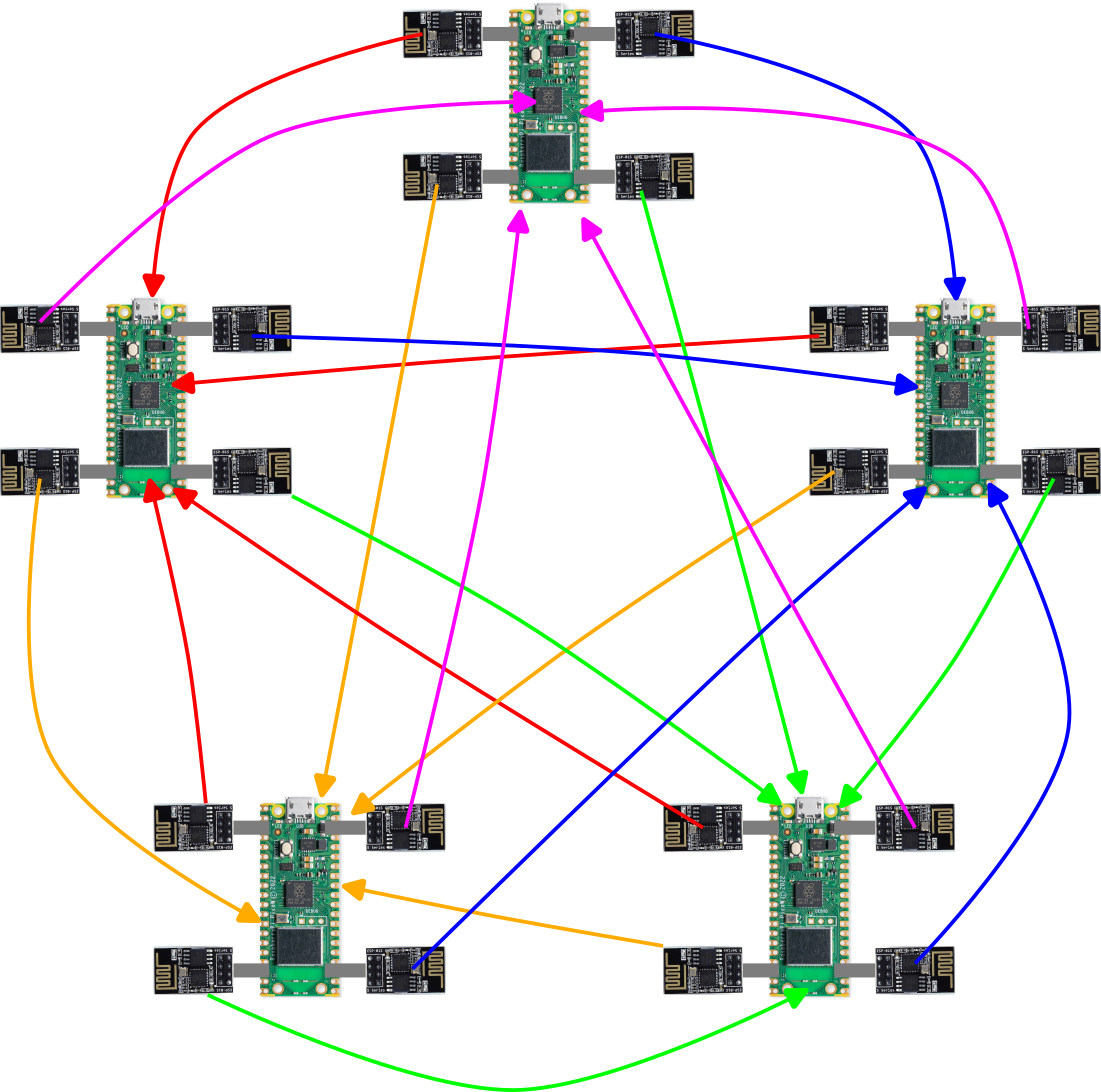
\includegraphics[width=0.8\linewidth]{connections}
  \caption{A fully connected mesh network consisting of five Raspberry Pi Pico W controllers,
  each equipped with four ESP-01 radio modules (plus its own internal Wi-Fi module).
  Each arrow represents a single Wi-Fi connection.
  All arrows of the same color are connected to a single central device. Information flows in the direction of the arrow.} 
  \label{fig:connections}
\end{figure}


\subsection{Simulator geometry}

Our simulator is designed in the context of the multi-agent planning problem,
and to simplify the planner's logic, such tasks typically deal with a discrete world (for example, divided into cells).
Additionally, when transferring this implementation to physical robots, they need to understand their position in space.
For this reason, we decided that the robots would move on a square grid, stopping at the intersections of the lines of this grid.

From the perspective of movement logic,
a robot can move forward or backward by a whole number of cells,
or turn left or right by a whole number of quarters.
This is implemented in the physical robot through a line sensor that tracks how many lines the robot has crossed forward or how many turns it has made.

The radio system simulation, on the other hand, cannot operate in discrete coordinates
because the propagation of radio signals must be isotropic,
meaning it is symmetric with respect to rotation\footnote{This is accurate for general-purpose antennas,
such as those found in Wi-Fi modules,
but there are also more directional antennas.
Our simulator can be used with an anisotropic signal strength profile as well.
Regardless, antennas never have a signal profile that follows a rectangular grid.},
but in discrete coordinates, it is impossible to draw a perfect circle.
For this reason, the simulation of radio communication occurs separately,
and while the robot moves from one cell to another,
the simulator continuously updates the signal strength value.
Each frame that any robot moves, the state of the radio system will be updated.

As a result, the logic within the robot is divided into two parts:
the chassis logic and the radio communication driver.
The interaction between these modules is synchronized using shared memory
(or more precisely, primitives like channels and semaphores that are based on shared memory),
while for the most part, they operate independently.
This can be achieved on multi-core microcontrollers, such as the Raspberry Pi Pico/RP2040 (our first choice for this project),
or by using asynchronous programming paradigms,
or it can be trivially accomplished with support for multiple processes within a kernel like Linux.

\subsection{API for User Code}

For the development of the simulator, we decided to use the Rust programming language.
It allows us to write fast and safe code that can be compiled
on many platforms without changes~\cite{10.1145/2663171.2663188}.
As a result, the simulator can be run as a native application on Linux or Windows, or as a web application via WebAssembly
\footnote{You can find the latest version of the simulator application at \texttt{https://mesh-playground.roboticlab.ru}:
it should run inside of any browser that supports WebAssembly and WebGL, which would be around 96\% of all browsers currently in use.}

This approach also enables the use of the same code within the simulator and on real hardware -- 
this will only require writing a driver for that hardware, and then the Rust code can be compiled for the embedded platform.

This driver is represented by a structure that implements the required trait
(which is analogous to an interface in Rust).
To support a particular platform, it is only necessary to implement the corresponding asynchronous methods~\footnote{For
embedded development in Rust, the popular Embassy project is used.
It allows writing asynchronous programs for supported embedded platforms
in a way that is even easier than writing traditional sync Rust code.
This differs from development on Arduino, for example,
where platform limitations often lead to code being written in a synchronous style in C++.}
to implement the functionality.

To control the movement of the chassis, we can define our own interface,
and at this moment (as mentioned earlier), the robot can move forward/backward by several cells or make several quarter turns left/right.
It also has the option to wait for a few seconds or to output a debug message (which will only be visible in the simulator).

For managing radio communication, we must consider the capabilities of the physical radio module.
The API only exposes those methods for which the ESP-01 has corresponding AT commands available:
for example, scanning for neighboring Wi-Fi networks, connecting to one of them, disconnecting,
and measuring signal strength. There is also a method to send a message to the robot to which we
are currently connected, in accordance with the radio communication model described above. These methods are detailed in listing \ref{code:traits}.

\begin{listing}[h]
\caption{Function signatures for the radio receiver and transmitter interfaces. The driver must implement these two interfaces to be compatible with our simulator.}
\label{code:traits}
\begin{minted}[fontsize=\footnotesize]{rust}
/// Interface for message receivers (Wi-Fi AP).
pub trait ReceiverNic<PeerId, MessageType> {
type Error: core::fmt::Debug;
  /// Retrieve a single message that was sent to this receiver.
  /// The driver has a limited buffer for messages, so
  /// if this is called infrequently,
  /// some messages may be lost.
  ///
  /// Asynchronously blocks until a message is received.
  async fn get(&mut self) -> Result<(PeerId, MessageType), Self::Error>;
  
  /// Gets the ID (e.g., MAC address) of this receiver.
  /// Senders will see me with this ID.
  async fn get_id(&mut self) -> Result<PeerId, Self::Error>;
}
  
/// Interface for transmitters. It can send messages to one other receiver,
/// but it must first be connected to it.
/// (Wi-Fi STA connected to AP).
pub trait TransmitterNic<PeerId, MessageType> {
  type Error: core::fmt::Debug;

  /// Checks that this transmitter is functioning.
  async fn ping(&mut self) -> Result<(), Self::Error>;

  /// Gets the receiver to which we are connected.
  /// Returns None if we are not connected.
  async fn get_peer(&mut self) -> Result<Option<PeerId>, Self::Error>;

  /// Gets the signal strength of the current connection.
  /// The signal strength may be 0 if we are currently out of range
  /// of the receiver,
  /// but are still connected to it in the module.
  /// It returns an error if there is no connection.
  async fn get_connection_info(&mut self) -> Result<ConnectionInfo<PeerId>, Self::Error>;

  /// Scans for available receivers. Returns the number of visible IDs.
  /// Found IDs are written to the provided array.
  /// If fewer receivers are visible than there is space in the array,
  /// the values of the last elements are undefined.
  /// If there are more receivers than space, then the first ones (as returned by the module) are written to the array.
  async fn scan(&mut self, peers: &mut [PeerId]) -> Result<usize, Self::Error>;
  
  /// Attempts to connect to one receiver.
  /// If it is in range and the connection is successful,
  /// returns Ok(()).
  async fn pair(&mut self, peer: PeerId) -> Result<(), Self::Error>;
  
  /// Attempts to disconnect from the receiver.
  /// Works even if the receiver is out of range.
  /// If we are not connected to the receiver, it does nothing.
  async fn unpair(&mut self) -> Result<(), Self::Error>;
  
  /// Sends a message to the connected receiver.
  async fn send(&mut self, message: MessageType) -> Result<(), Self::Error>;  
}
\end{minted}
\end{listing}

Finally, the two parts of the control run in separate threads
(using the game-engine async utils in the simulator and via \texttt{\#[embassy::task]} on the physical platform).
There is a communication channel between them to allow the threads to inform each other of interesting events
(for example, if I want to send a message to another robot,
or the mesh network has delivered me a message).

\begin{figure}
  \centering
  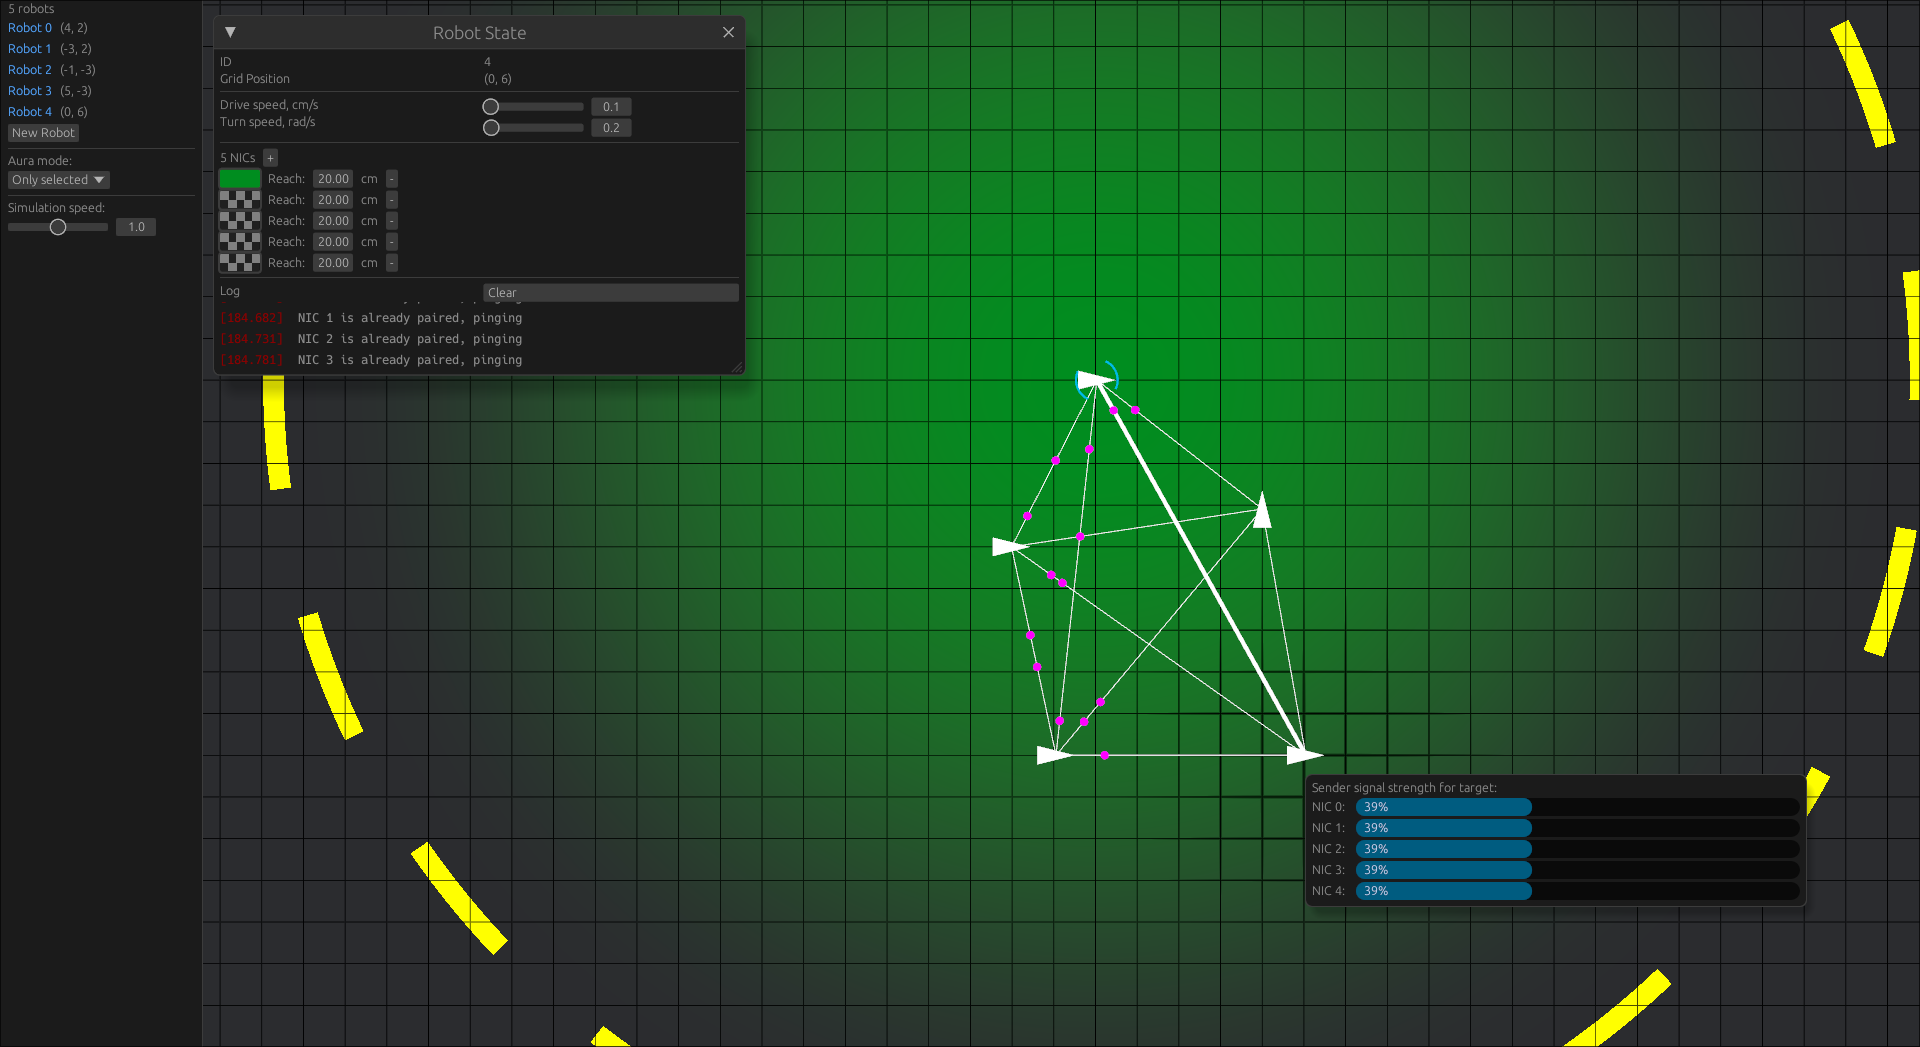
\includegraphics[width=0.8\linewidth]{simulator-connections}
  \caption{The mesh network, depicted in Figure \ref{fig:connections}, implemented within the simulator. Each robot has four virtual interfaces that allow them to establish connections with each of their neighbors. The aura and dashed circle around the top robot indicate the range of its radio interfaces; the signal strength indicator shows that the connection between the top robot and the bottom-right robot has a strength of 39\%. Circles on the connections represent radio messages in-flight between the robots: these have been sent but not yet delivered.}
  \label{fig:simulator-connections}
\end{figure}


\subsection{Memory limitations in microcontrollers (and their effects on our design)}

Many embedded systems have very small limits on RAM and other resources,
especially compared to regular computers. For example, the Raspberry Pi Pico,
which we are focusing on in this project,
has 264KB of RAM and only 2MB of flash memory~\cite{raspberrypi2021}
(of which only 1MB can be used if you want to use over-the-air (OTA) updates,
because OTA requires storing the new version of the firmware while the old is still running).

Due to this, there is a priority in designing our interfaces to use as little RAM as possible.
This can be seen in some architectural decisions:
for example, when scanning for Wi-Fi networks,
we do not return a \texttt{Vec} of found networks --
because that would require using dynamic memory,
and an attacker could create a large number of Wi-Fi networks which will overrun the available memory when doing a scan.
Instead, the scanning routine takes a pointer to a buffer where it stores information about the networks:
if the number of available networks exceeds the size of the buffer,
only the first few networks are saved in the buffer, while the rest are ignored.

Similarly, many application architecture decisions are made at compile time rather than at runtime.
For instance, the firmware has a fixed number of Wi-Fi modules that a single robot can support,
and after compilation, no additional modules can be connected to the Raspberry Pi Pico.
(You can still use fewer with the same firmware binary image, because all operations with the Wi-Fi module can return an error
(so the user code already must deal with them appropriately),
and one possible error condition is that the module is unresponsive or not connected.
However, checking the modules takes time that could potentially be saved.)

In cases where the single RPi Pico's memory is not enough,
\emph{hardware offloading} can be performed:
by default, we use the ESP-01 modules as "black boxes,"
communicating with them solely through AT commands defined by their default firmware.
However, the ESP8266 processor that they use contains 50KB of RAM --
and, perhaps more importantly, it supports up to 16MB of program memory via SPI.
Therefore, one can write a special firmware for these modules that offloads
some aspects of network operation beyond the main controller's code,
allowing the main controller to send higher-level commands to the ESP,
thereby saving program memory for these more complex operations.
(Another benefit is that lookup tables and additional data structures
which can be precompiled can be stored in the extra space on the ESP's flash,
and retrieved by the main controller when needed;
however, in the algorithms we've researched, there
does not appear to be a significant need for large static data structures.)

This is also beneficial because it increases the number
of processor cores available for various operations:
the RPi Pico has just two cores, but if one decides to use the cores of the ESP8266,
then the system will have a total of 6 cores.
However, these are limited in their communication capabilities:
if one ESP wants to send a message to another,
then a naive approach would be for the first ESP to wait for the RPi to query it, and only after that will the RPi relay the message to the other ESP.

A more complex scheme can be employed,
where different bus participants can send messages to each other
without the involvement of a central controller (for example, the PCI bus works this way), but this is more complicated:
PCI uses a separate chip, called a "bus arbiter",
to regulate which of the bus participants can begin a transaction.

In any case, this approach requires writing special firmware for the ESP-01,
which can be difficult -- our simulator does not support this,
and implementing such support would essentially mean creating a virtual machine for each type of microcontroller.

Finally, if the resources of the microcontrollers are completely insufficient,
one can simply use a more powerful controller,
such as the Raspberry Pi Zero: this is a full-fledged Linux computer with 512MB of RAM.
Compared to microcontrollers, this will allow for the execution of very complex programs.


\subsection{Simulator architecture}

Since we chose Rust as the primary development language,
we decided to use Bevy -- a game engine based on the ECS (Entity-Component-System) model.
In this model, there are \emph{entities} that have only a unique identifier.
One or more \emph{components} are attached to them, which describe some state:
for example, in the simulator, one of the components indicates that a given entity is a robot that is currently moving from one cell to another.
Finally, \emph{systems} are called in a loop—functions that process and modify the data in the components.

This architecture is similar to that used in more popular game engines
like Unity~\cite{unity} and Godot; however, in those engines, components
and systems are combined into a single thing
(in Unity, the base class for this is called \texttt{MonoBehaviour}).
This design performs worse in situations where one piece of code needs
to operate on multiple different objects
(for example, in the radio simulations in this project)
and often requires the creation of additional virtual objects just to hold the code for such coordination.


\section{Conclusion}

In this work, we developed a simulator for wireless mobile mesh networks and demonstrated its API.
Based on this API, algorithms can be implemented that will run 
on both simulated and hardware platforms,
without having to change the code.
This is a novelty to the field of network architecture modeling,
which has previously focused more on the challenges of modeling fixed networks.

Due to the flexibility of the Rust language,
the interface we provide for user code can be utilized across various microcontrollers.
As a result, we can expect that working with our simulator will serve as
a foundation for future mesh networking solutions that support different microcontrollers and physical interfaces.

\subsection{Future work}

Our simulator is primarily designed for interactive use, requiring a graphical user interface (GUI).
As a result, it is unsuitable for situations where a GUI is not available, such as on servers or HPCs/supercomputers.
It is also limited by the speed of the game engine, which is currently set to 60 frames per second:
many events require at least one frame of simulation
to pass between an event and a reaction
(for example, each transaction between the radio module code and
the virtual radio module requires one frame to be accepted by the simulator).
Because of this, even if the message transmission speed is set to infinity,
one robot will still not be able to send more than 60 messages per second to another robot.

These limitations are related to the specific implementation of the
simulator based on the Bevy game engine,
not to any particular issue with the interface or the concept itself.
In the future, we plan to create an optional implementation that will operate
without a graphical interface and handle events in discrete time:
such a version will allow for the simulation of much larger networks,
and will potentially be capable of distributed computation.

For use in the context of the multi-agent planning problem,
the simulator will be enhanced with functions to create additional objects
with which the robots can interact:
right now the robots can only drive around an empty environment.
If they had something to do, like picking up boxes,
then it would enable seeing how the routing algorithm and the planning algorithm work together.


%Заключение является неотъемлемой частью любой работы. 

%Оно должно содержать краткие выводы по результатам исследования,
%отражающие новизну и практическую значимость работы, предложения по
%использованию ее результатов, оценку её эффективности и качества.

% \section{Ethical disclaimers}

% A disclaimer is a note of disclaimer of responsibility~\cite{kulyabov_2024_editorial_author-ethics_en}.
% For example, authors' statements about conflicts of interest, author contributions, acknowledgements, etc.

% Authors should not prepare these disclaimers as a numbered or unnumbered
% \mintinline{latex}{\section}%
% ; please use the special environments instead.

% \subsection{Author contributions}

% The Committee on Publication Ethics (COPE) draws attention to the problem of authorship \cite{cope_book_authorship_en}.
% The CRediT system (\url{https://credit.niso.org/}) is proposed to formalize author roles.
% The CRediT (Contributor Roles Taxonomy) offers 14 possible author roles \cite{holcombe_2019_contributorship-not-authorship_en}.
% This is not really a taxonomy, but a faceted classification. Author roles are not always independent in themselves.

% The following statements should be used \emph{Conceptualization, X.X. and Y.Y.; methodology, X.X.; software, X.X.; validation, X.X., Y.Y. and Z.Z.; formal analysis, X.X.; investigation, X.X.; resources, X.X.; data curation, X.X.; writing---original draft preparation, X.X.; writing---review and editing, X.X.; visualization, X.X.; supervision, X.X.; project administration, X.X.; funding acquisition, Y.Y.}
% Please add at the end of the statement:
% \emph{All authors have read and agreed to the published version of the manuscript.}

% This section has a special environment:
% \begin{minted}{latex}
% \begin{authorcontributions}
% …
% \end{authorcontributions}
% \end{minted}

% \subsection{Funding}

% Disclaimer \emph{funding} refers primarily to external funding if the research was externally initiated.
% If the research is entirely the initiative of the author's team, it is better to indicate gratitude for partial funding of some of the stages of the research in the \emph{Acknowledgments} section.
% The fact that the author's team has received external funding should be recorded in the disclaimer as a matter of course.
% When mentioning the sponsor, its exact data (name of the organization, grant number, etc.) and the country of its location should be specified (for example \emph{This research was funded by NAME OF FUNDER grant number XXX}).
% If there is any support, it is recommended to clarify in the \emph{Conflicts of interest} section at which stages of the research and how the support was used.
% If there is no external funding, it is written: \emph{This research received no external funding}.
% If it is impossible to obtain information from the authors about the source of funding, then write: \emph{Not specified}.

% This section has a special environment:
% \begin{minted}{latex}
% \begin{funding}
% …
% \end{funding}
% \end{minted}

% \subsection{Data availability statement}

% Data are particularly important in reproducible researches.
% The data availability statement tells the reader where the research data related to the article are located and under what conditions the data can be accessed.
% References to the dataset are also provided.

% If no new data is created or analyzed, please write:
% \emph{No new data were created or analyzed in this study. Data sharing is not applicable.}

% This section has a special environment:
% \begin{minted}{latex}
% \begin{dataavailability}
% …
% \end{dataavailability}
% \end{minted}

% \subsection{Conflicts of interest}

% This disclaimer must be included.

% Conflicts of interest can comment on various aspects, but usually the author's past or current employment is indicated.
% Grants (especially from for-profit companies) received not only by the author but also by the organization for which he or she works are indicated.
% If the author is associated with a sponsor, it is indicated where the research was conducted.

% If there is no conflict of interest, then the corresponding statement should also be included: \emph{The authors declare no conflict of interest}.

% This section has a special environment:
% \begin{minted}{latex}
% \begin{conflictsofinterest}
% …
% \end{conflictsofinterest}
% \end{minted}

% \subsection{Acknowledgments}

% Identification of funding sources and other support, and thanks to individuals and groups that assisted in the research and the preparation of the work should be included in an acknowledgment section, which is placed just before the reference section in your document.

% This section has a special environment:
% \begin{minted}{latex}
% \begin{acknowledgments}
% These are different acknowledgments.
% \end{acknowledgments}
% \end{minted}
% so that the information contained therein can be more easily collected during the article metadata extraction phase, and to ensure consistency in the spelling of the section heading.

% \section{Appendices}

% If your work needs an appendix, add it before the
% \mintinline{latex}{\end{document}}
% command at the conclusion of your source document.

% Start the appendix with the
% \mintinline{latex}{\appendix}
% command:
% \begin{minted}{latex}
% \appendix
% \end{minted}
% and note that in the appendix, sections are lettered, not numbered.

\newpage

% \begin{authorcontributions}
% %  Концептуализация, написание --- рецензирование и редактирование: Анна Владиславовна Королькова; методология, написание --- подготовка первоначального варианта: Дмитрий Сергеевич Кулябов.
% Концептуализация, написание --- подготовка первоначального варианта: Генералов Даниил Михайлович;
% руководство, написание --- рецензирование и редактирование: Андрей Николаевич Виноградов.
%   Все авторы прочитали и согласились с опубликованной версией рукописи.
% \end{authorcontributions}

% \begin{funding}
%   Данное исследование не получало внешнего финансирования.
% \end{funding}

% \begin{dataavailability}
%   В ходе исследования не было создано и проанализировано никаких новых данных. Совместное использование данных неприменимо.
% \end{dataavailability}

% \begin{conflictsofinterest}
%   Авторы заявляют об отсутствии конфликта интересов.
% \end{conflictsofinterest}

%\begin{acknowledgments}
%  Мы благодарим организаторов конференции за предоставленную возможность создать этот шаблон.
%\end{acknowledgments}

%%
%% Define the bibliography file to be used

\section{References}

\printbibliography[heading=none]

%%
%% If your work has an appendix, this is the place to put it.
%\appendix

%\section{Онлайн-ресурсы}

%\begin{itemize}
%\item Overleaf: \url{https://www.overleaf.com/read/vjvjpsqrqjhj#86e97e}.
%\item Overleaf (russian): \url{https://www.overleaf.com/read/yjmkpnvgqzdk#bf8ccf}.
%\end{itemize}

\end{document}

%%% Local Variables:
%%% mode: LaTeX
%%% TeX-master: t
%%% End:
